\documentclass[nooutcomes]{ximera}
%% handout
%% space
%% newpage
%% numbers
%% nooutcomes

%I added the commands here so that I would't have to keep looking them up
%\newcommand{\RR}{\mathbb R}
%\renewcommand{\d}{\,d}
%\newcommand{\dd}[2][]{\frac{d #1}{d #2}}
%\renewcommand{\l}{\ell}
%\newcommand{\ddx}{\frac{d}{dx}}
%\everymath{\displaystyle}
%\newcommand{\dfn}{\textbf}
%\newcommand{\eval}[1]{\bigg[ #1 \bigg]}


\newcommand{\RR}{\mathbb R}
\renewcommand{\d}{\,d}
\newcommand{\dd}[2][]{\frac{d #1}{d #2}}
\renewcommand{\l}{\ell}
\newcommand{\ddx}{\frac{d}{dx}}
\newcommand{\dfn}{\textbf}
\newcommand{\eval}[1]{\bigg[ #1 \bigg]}

\usepackage{multicol}

\renewenvironment{freeResponse}{
\ifhandout\setbox0\vbox\bgroup\else
\begin{trivlist}\item[\hskip \labelsep\bfseries Solution:\hspace{2ex}]
\fi}
{\ifhandout\egroup\else
\end{trivlist}
\fi} %% we can turn off input when making a master document
\usepackage{fullpage}

\title{3.6 Derivatives as Rates of Change}  

\begin{document}
\begin{abstract}		\end{abstract}
\maketitle


%problem 1
\begin{problem}
The graph of $s=f(t)$ is the position of John walking along a straight path.


	\begin{image}
	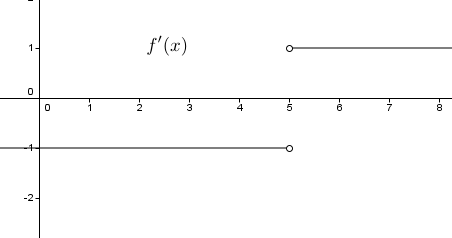
\includegraphics[scale=.4]{Figure13.png}
	\end{image}

	\begin{image}
	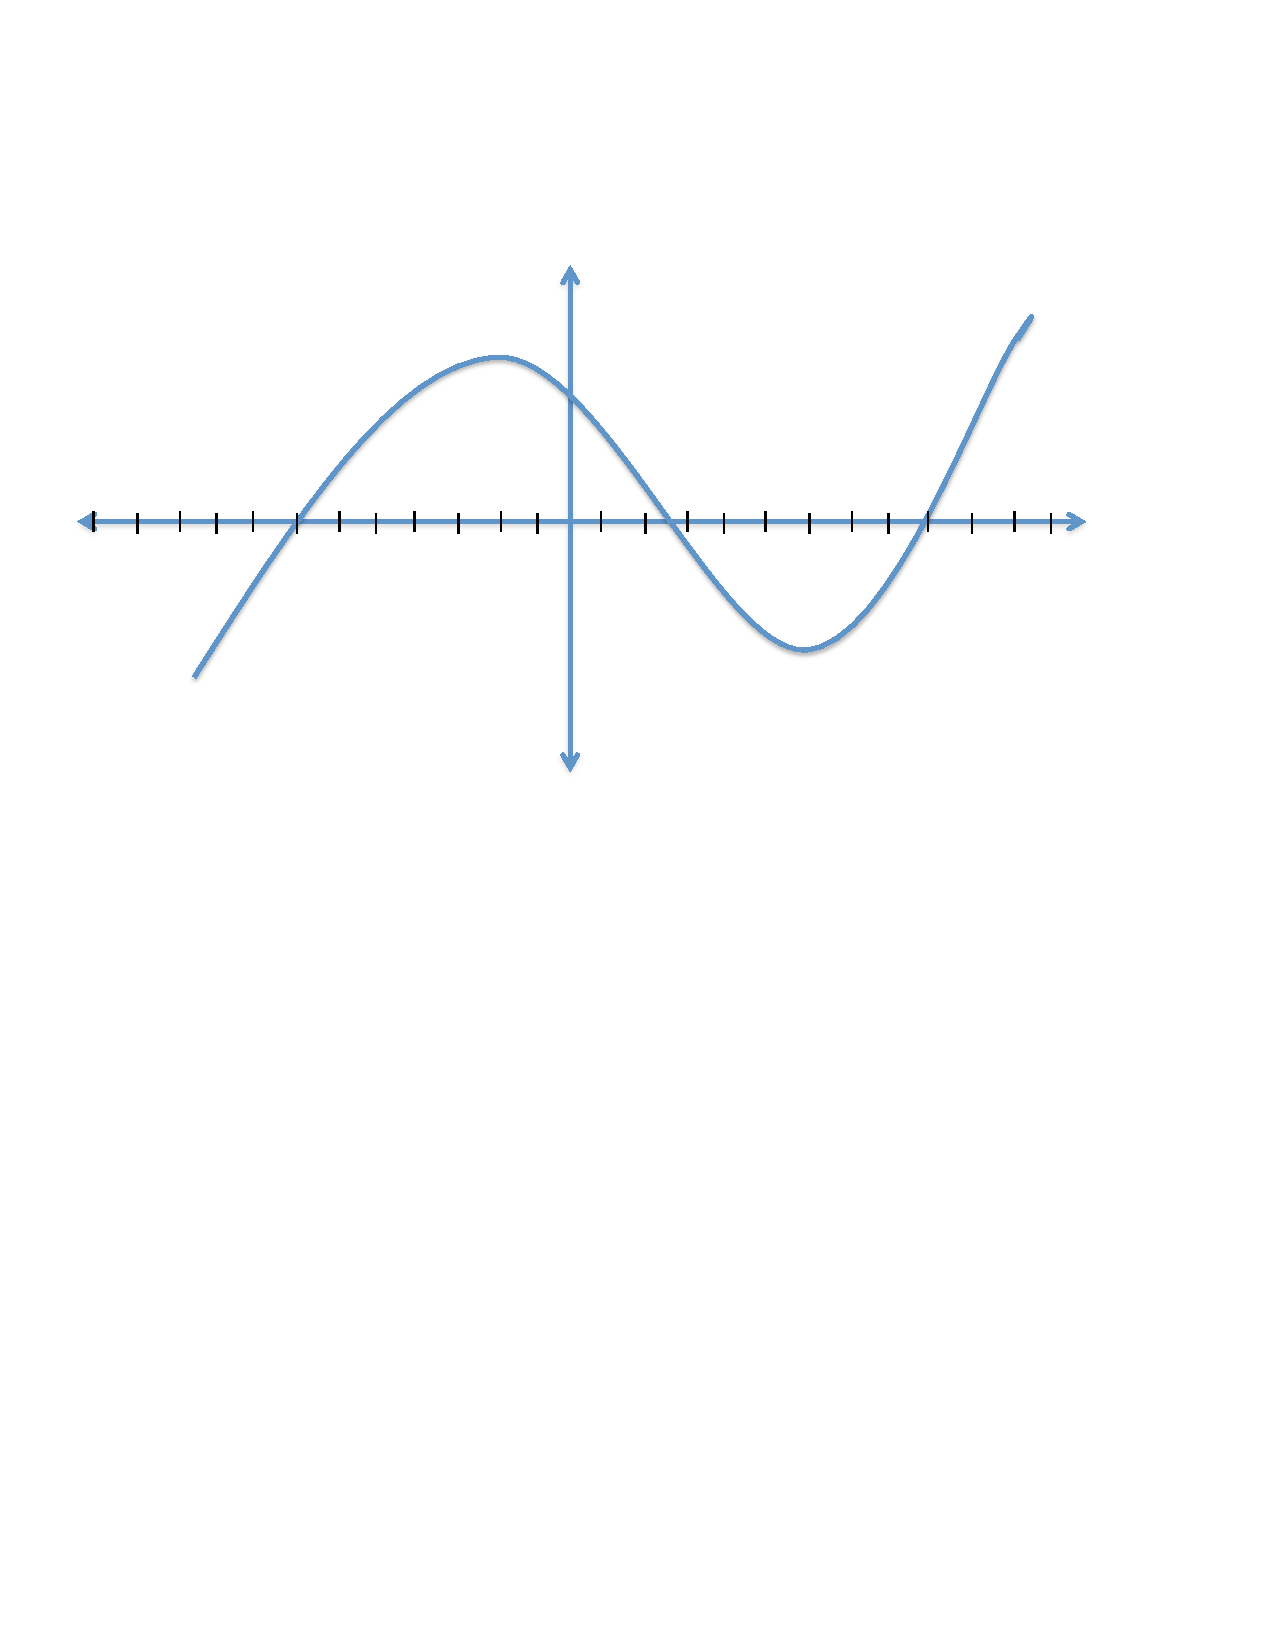
\includegraphics[trim= 140 420 290 180]{Figure2.pdf}
	\end{image}
	
	\begin{enumerate}
	
	%part a
	\item  Describe the motion of the object as precisely as you can.
		\begin{freeResponse}
		Let us assume that $f(t)$ gives the position of John from his house at time $t$.  If $f(t) < 0$, then John is west of his house;  if $f(t) > 0$, then John is east of his house; if $f(t)=0$, then John is in front of his house.  
		
		For the first hour, that is, for $0 \leq t \leq 1$, John walks east away from his house.
		
		\begin{image}
		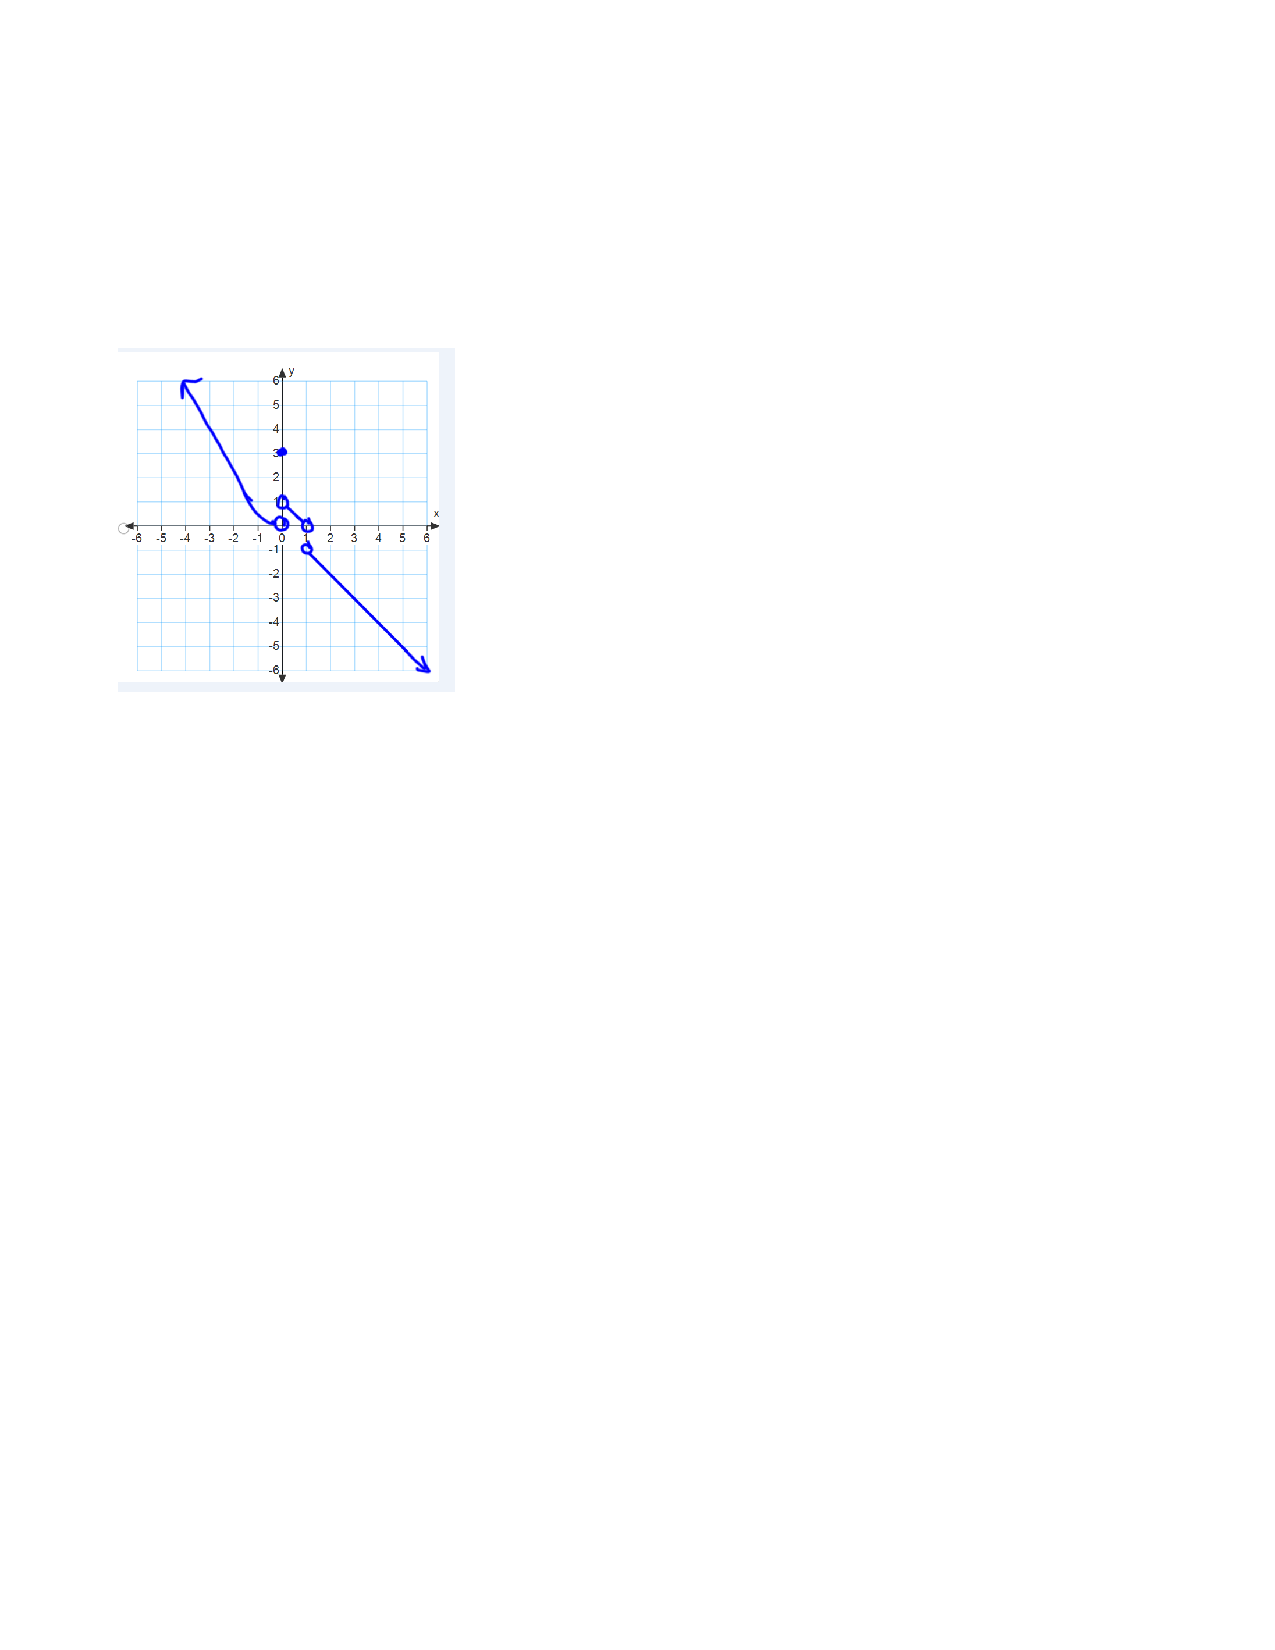
\includegraphics[trim= 140 570 290 200]{Figure3.pdf}
		\end{image}
	
		For the second hour, that is, for $1 \leq t \leq 2$, John turns around and starts walking back west.  However, he does not walk all the way back to his house.
		
		\begin{image}
		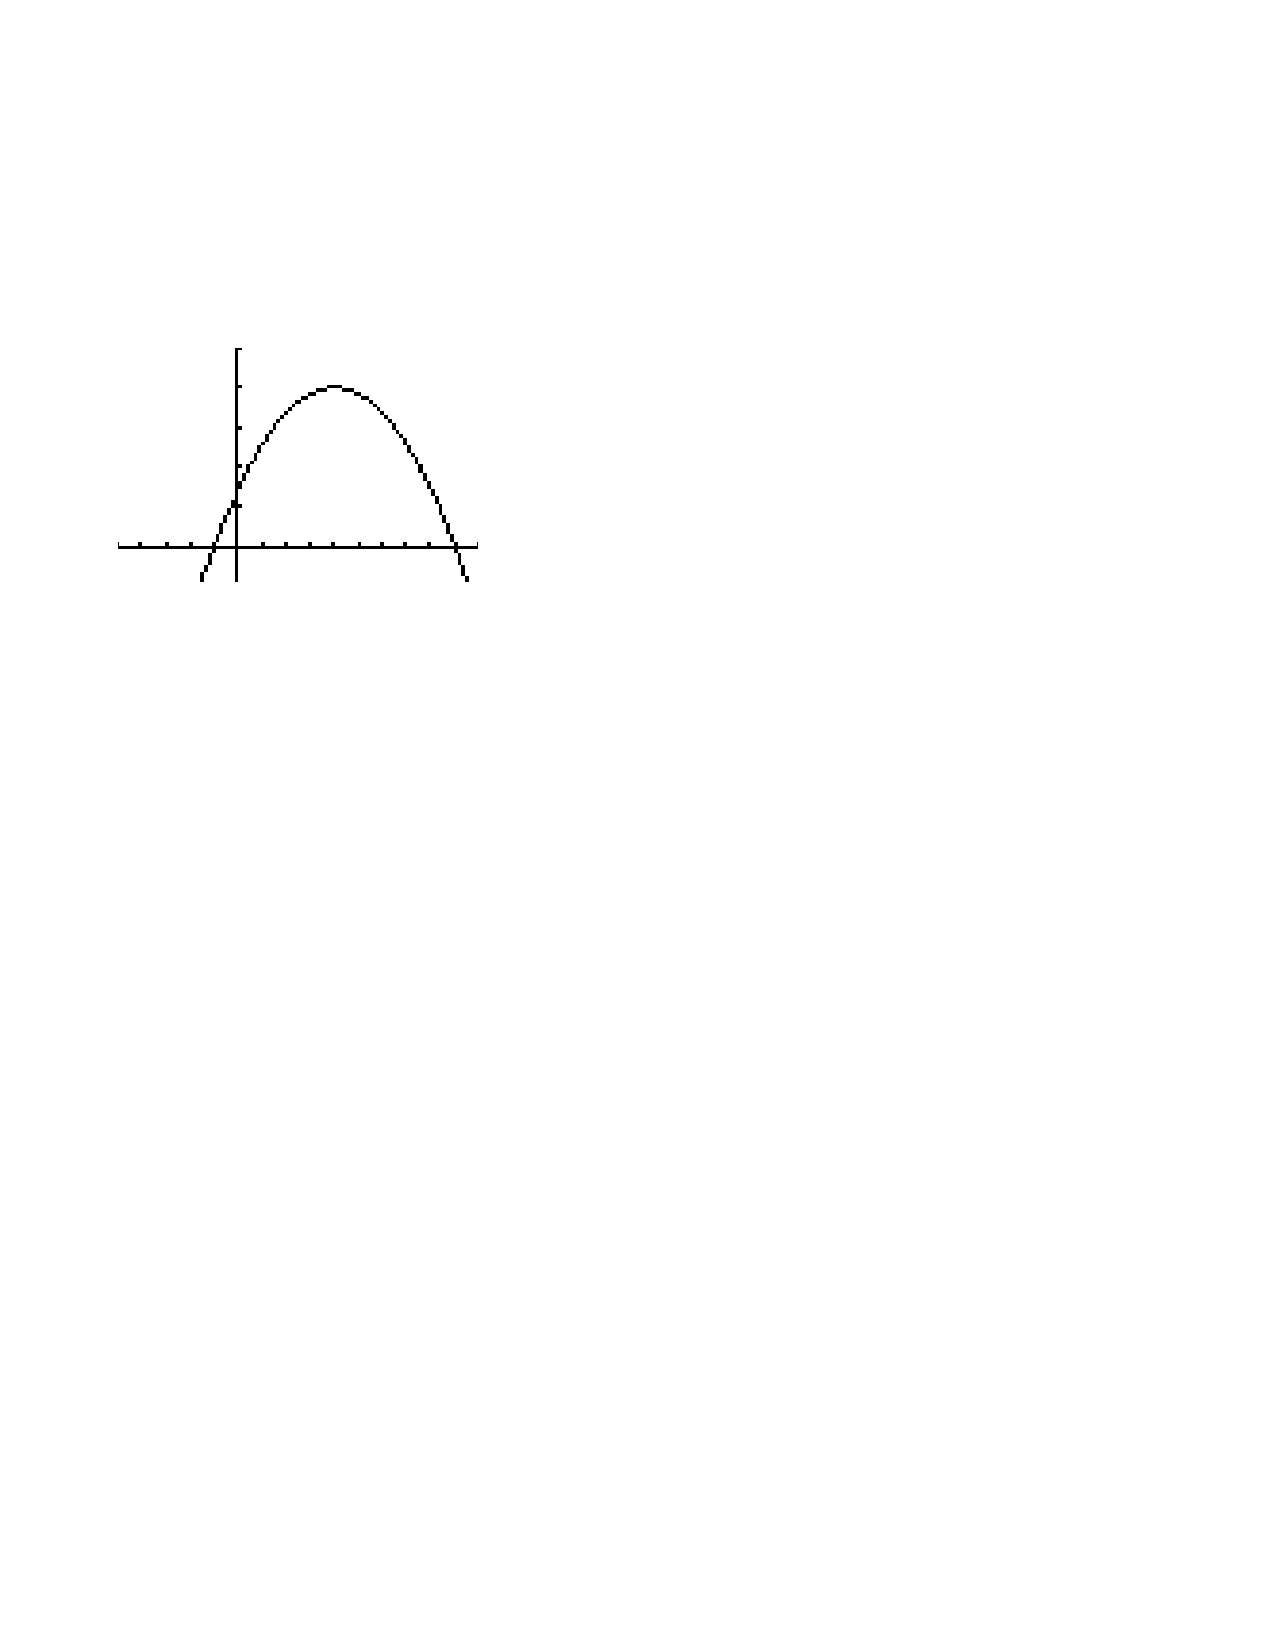
\includegraphics[trim= 140 570 290 200]{Figure4.pdf}
		\end{image}
		
		For the third hour, that is, for $2\le t\le 3$, John realizes he needs to pick up an apple from the grocery store, which is way east of his house, for Elaine.  So he turns around again and walks east to the store.
		
		\begin{image}
		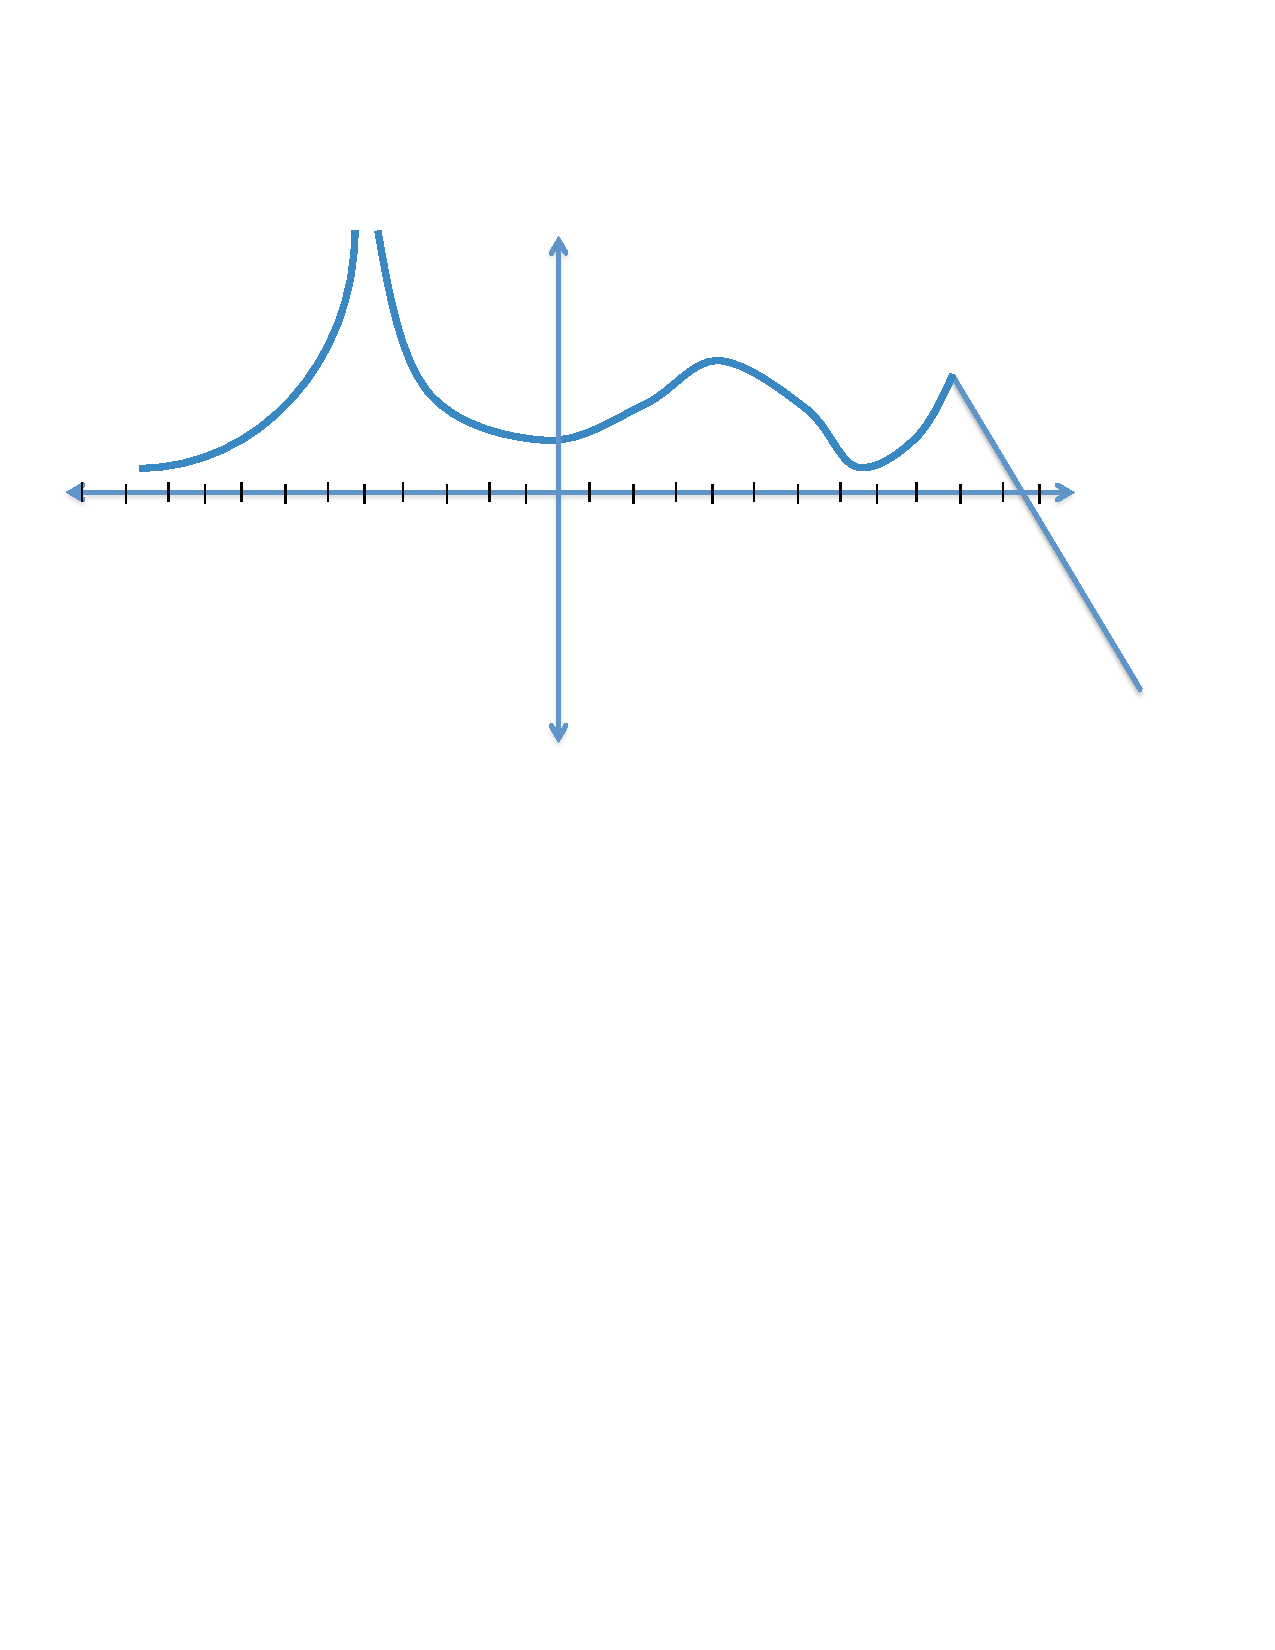
\includegraphics[trim= 140 570 290 200]{Figure5.pdf}
		\end{image}
		
		For the fourth hour, that is, for $t \ge 3$, John needs to drop the apple off at Elaine's house, which is west of his house.  He turns west and walks past his house until he makes it to Elaine's house.
		
		\begin{image}
		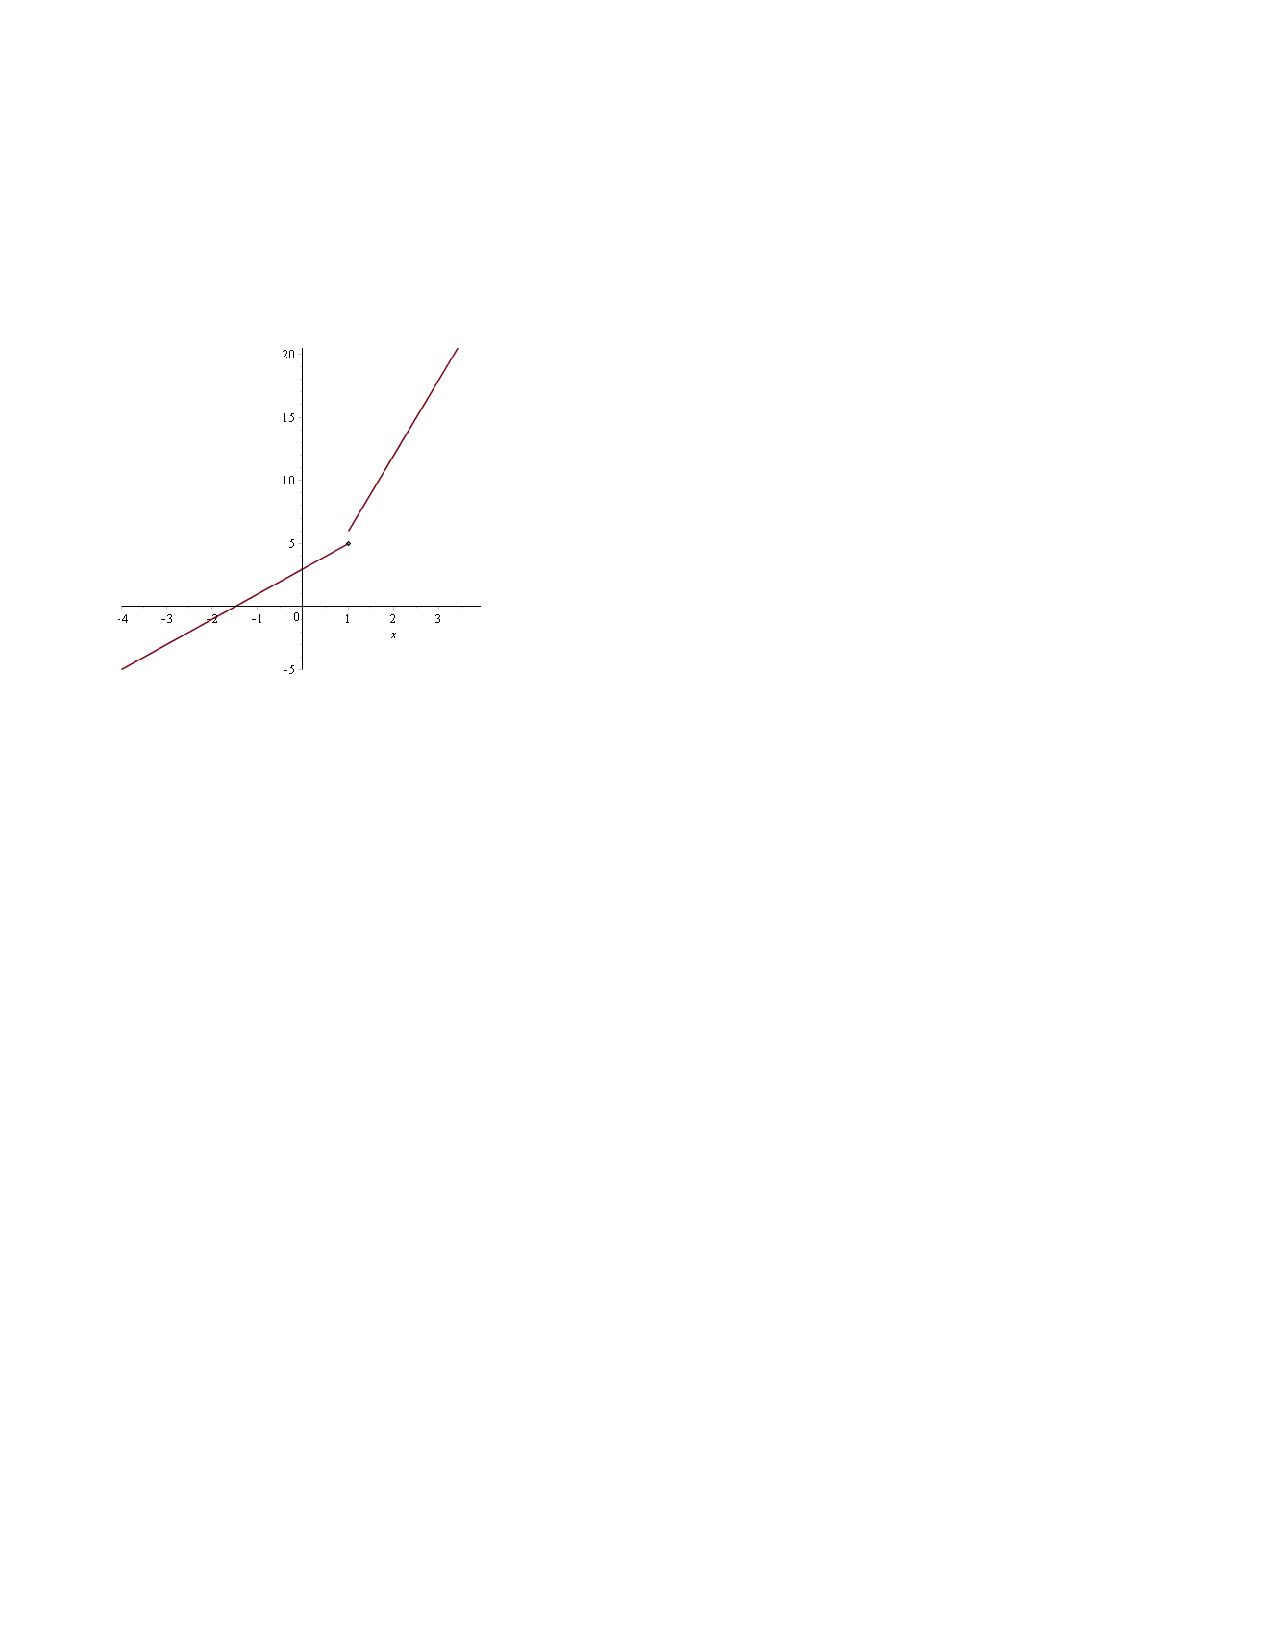
\includegraphics[trim= 140 540 290 200]{Figure6.pdf}
		\end{image}

		\end{freeResponse}
		
		
		
	%part b
	\item  When is the velocity of the object zero?  What is happening to the object at those times? 
		\begin{freeResponse}
		John's velocity is zero at times $t=0,t=1,t=2$, and $t=3$ (the times where the slopes of the tangent lines are zero).  At these times, John changes direction since the slopes of the tangent lines to the graph of $f(t)$ change from positive to negative.
		\end{freeResponse}
		
		
		
	%part c
	\item  When is the object moving in the positive direction?  When is the object the furthest in the positive direction and the furthest in the negative direction?
		\begin{freeResponse}
		John is moving in the positive direction (in this story, east) during times in the region $(0,1) \cup (2,3)$.  John is furthest in the positive direction at time $t=3$ and furthest in the negative direction at (approximately) time $t=3.5$.
		\end{freeResponse}
		
		
		
	%part d
	\item  When is the object speeding up and slowing down? When is the object going at maximum velocity?
		\begin{freeResponse}
		John is speeding up in the region $(0,0.5) \cup (1, 1.5) \cup (2, 2.5) \cup (3, 3.5)$.  He is slowing down in the region $(0.5, 1) \cup (1.5, 2) \cup (2.5, 3)$.  John is moving the fastest at time $t = 3.5$, but that maximizes his speed, not his velocity, because he is moving in the negative direction at that time.  It appears that he maximizes his velocity at about $t=2.5$.  
		\end{freeResponse}
		
		
		
	\end{enumerate}
			
			
	
\end{problem}





%problem 2
\begin{problem}
Suppose that a stone is thrown vertically upward from a cliff on Mars with an initial velocity of $64$ ft/s from a height of $192$ ft.  The height $s$ of the stone above the ground after $t$ seconds is given by $s(t) = -6t^2 + 24t + 192$.

	\begin{enumerate}
	
	%part a
	\item  Determine the velocity and acceleration of the stone after $t$ seconds.
			\begin{freeResponse}
			The velocity $v(t)$ is:  $v(t) = s'(t) = -12t + 24$.
			
			The acceleration $a(t)$ is:  $a(t) = v'(t) = s''(t) = -12$.
			\end{freeResponse}
			
			
			
	%part b
	\item  What is the greatest height of the stone and when does it occur?  What are the velocity and acceleration at that time?
			\begin{freeResponse}
			Since the function $s(t)$ is differentiable everywhere (it is a polynomial), the maximum height must occur at a time when the velocity is $0$.  So we solve:
			\begin{align*}
			v(t) = -12t+24 &:= 0 \\
			12t &= 24 \\
			t &= 2
			\end{align*}
			
			It is easy to check that $v(t) > 0$ for $0 \leq t < 2$ and $v(t) < 0$ for $2 < t$, and so the greatest height of the stone really does occur at time $t=2$.  The greatest height is $s(2) = -24 + 48 + 192 = 216$ ft.  For the second question we have already seen that $v(2) = 0$ ft/sec, and we have a constant acceleration of $-12$ ft/sec$^2$.  So $a(2) = -12$ ft/sec$^2$.
			\end{freeResponse}
			
			
			
	%part c
	\item  When does the stone hit the ground?  What are the velocity and acceleration at that time?
			\begin{freeResponse}
			The stone hits the ground when $s(t) = 0$.  So we solve:
			\begin{align*}
			s(t) = -6t^2 + 24t + 192 &:= 0 \\
			-6(t^2 - 4t - 32) &= 0 \\
			-6(t-8)(t+4) &= 0 
			\end{align*}
			
			Since we are only considering $t \geq 0$, we must have $t=8$.  At this instant, $v(8) = -96 + 24 = -72$ ft/sec and $a(8) = -12$ ft/sec$^2$.  
			
			\end{freeResponse}
			
			
			
	\end{enumerate}
			
			
			
		
\end{problem}

%problem3	
\begin{problem}	
	\begin{enumerate}
	
	%part a
	\item  True or False:  If the acceleration of an object is constant, then its velocity is constant.

		\begin{freeResponse}
		This is false in general, and is true if and only if the acceleration is 0.  Let $a$ denote your non-zero constant acceleration.  If $a > 0$ then your velocity is increasing, and if $a < 0$ then your velocity is decreasing.  See the accompanying picture for when $a>0$ (note that the units for $v(t)$ and $a(t)$ are \dfn{not} the same!)
		
			\begin{image}
			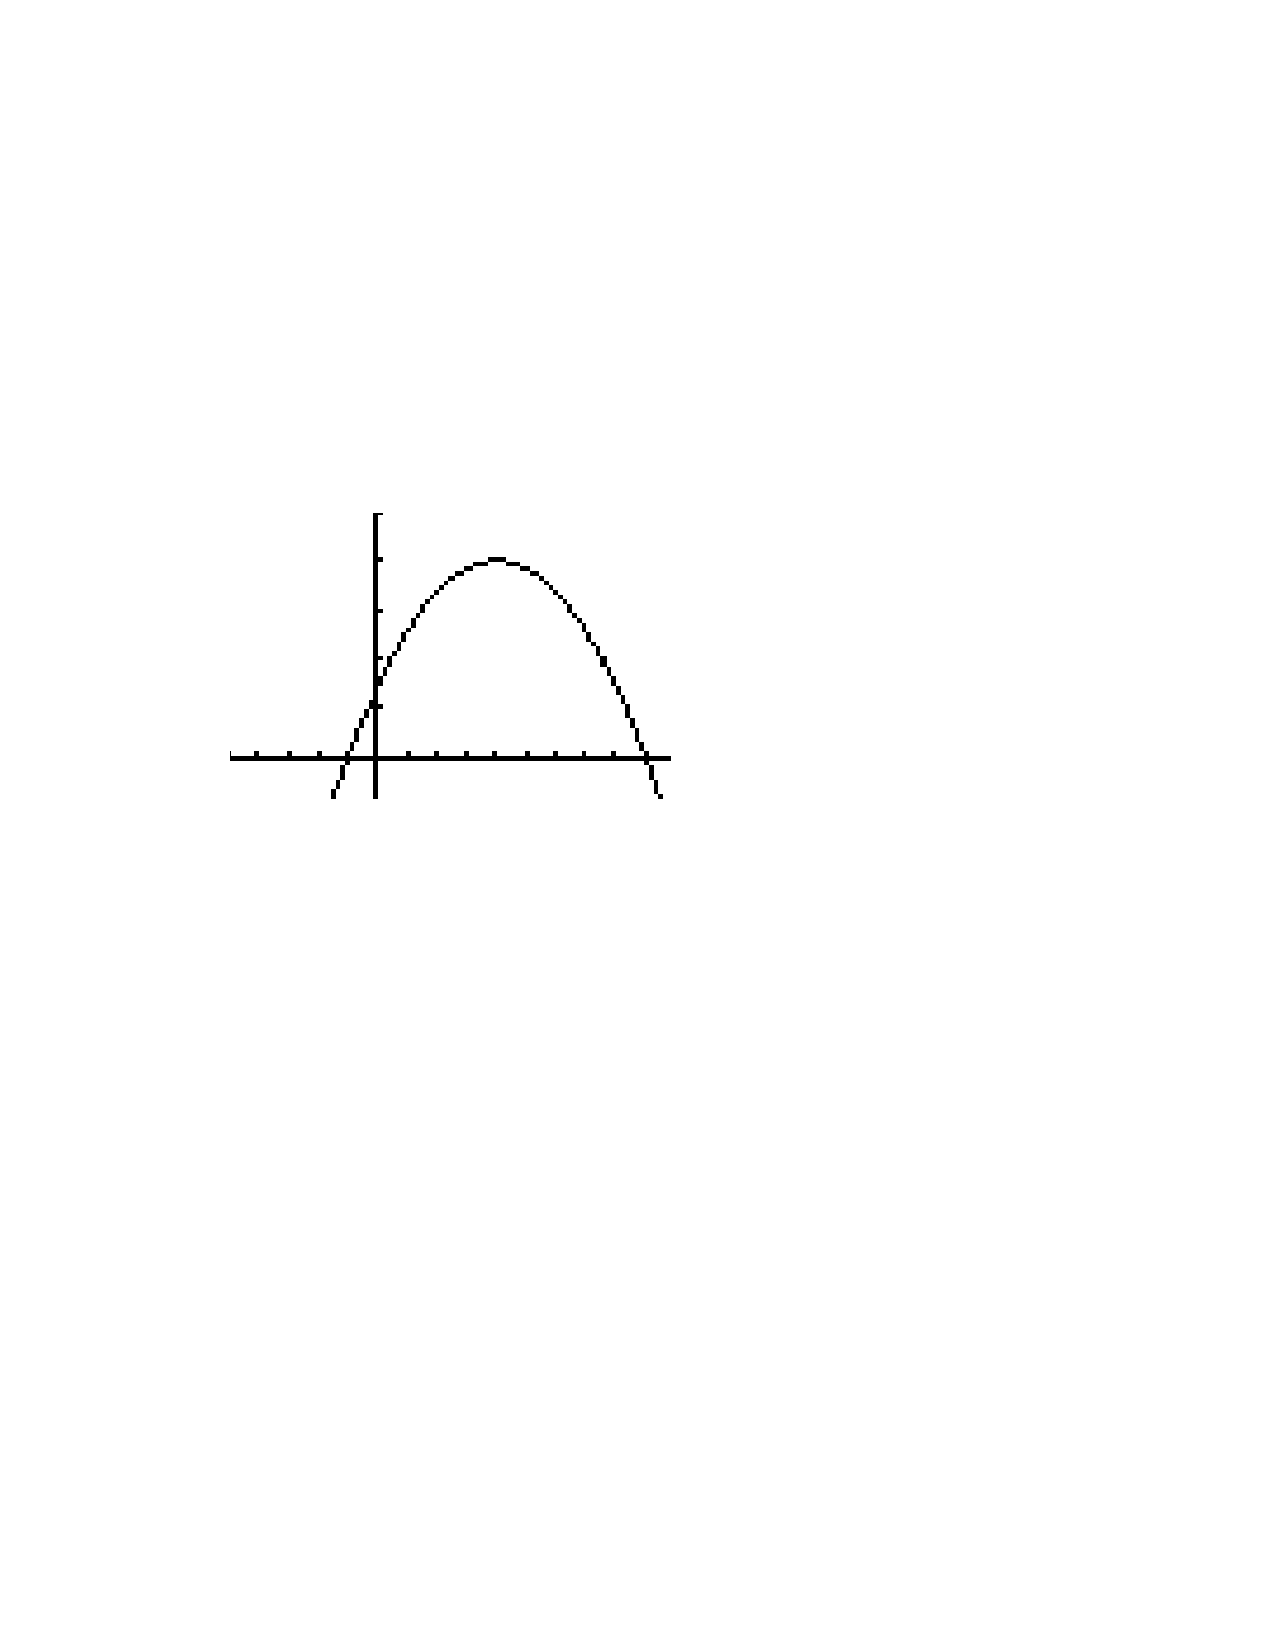
\includegraphics[trim= 170 420 250 180]{Figure1.pdf}
			\end{image}
		\end{freeResponse}	
		
		
	
	%part b	
	\item  True or False:  A moving object can have negative acceleration and increasing speed.

		\begin{freeResponse}
		True.  If your velocity is negative (which means that you are moving in the negative direction) then a negative acceleration increases the magnitude (or absolute value) of the velocity.  But the magnitude of the velocity is the speed.
		\end{freeResponse}	
		
		
		
	\end{enumerate}
	
	
\end{problem}	
	
%problem4
\begin{problem}
Suppose the average cost of producing 300 cellphones is 2 dollars per cellphone and the marginal cost at $x=300$ is 1.85 dollars per cellphone.  Interpret these costs.

	\begin{freeResponse}
		The first 300 cellphones costs, on average, 2 dollars to produce.  The 301st cellphone costs 1.85 dollars to produce.
	\end{freeResponse}

\end{problem}
	
%problem5
\begin{problem}
The total number of people, $N$ who have contracted a common cold by a time $t$ days after its outbreak on an island is given by $N=N(t)= \frac{200000}{1+100e^{-0.1t}},t\geq0$.

	\begin{enumerate}
		\item Evaluate and interpret the limit $\lim_{t \to \infty} N(t)$
			\begin{freeResponse}	
			$\lim_{t \to \infty} N(t)=\lim_{t \to \infty} \frac{200000}{1+100e^{-0.1t}}=200000$.  In the long run, 200000 people will get the cold.
			\end{freeResponse}
		\item How long will it take for the number of people who have contracted the cold to reach 40,000?
			\begin{freeResponse}
				\begin{align*}
				N(t)&=40000\\
				\frac{200000}{1+100e^{-0.1t}}&=40000\\
				200000&=40000(1+100e^{-0.1t})\\
				1+100e^{-0.1t}&=\frac{200000}{40000}\\
				100e^{-0.1t}&=5-1\\
				e^{-0.1t}&=\frac{4}{100}\\
				-0.1t&=\ln(.04)\\
				t&=\frac{\ln(0.04)}{-0.1}=32.1888
				\end{align*}
			It will take 33 days for the numbe rof people who have contracted the cold to reach 40,000.
			\end{freeResponse}
		\item The graph of the function $N$ on the interval $[0,100]$ is given below.  Sketch (as best you can) the graph of its derivative, $N'(t)$.
			\begin{image}
			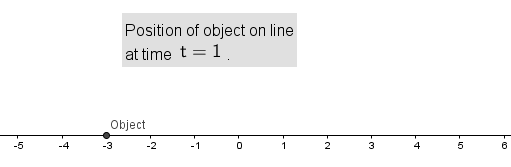
\includegraphics[scale=.4]{Figure8.png}
			\end{image}
				\begin{freeResponse}	
				\begin{image}
			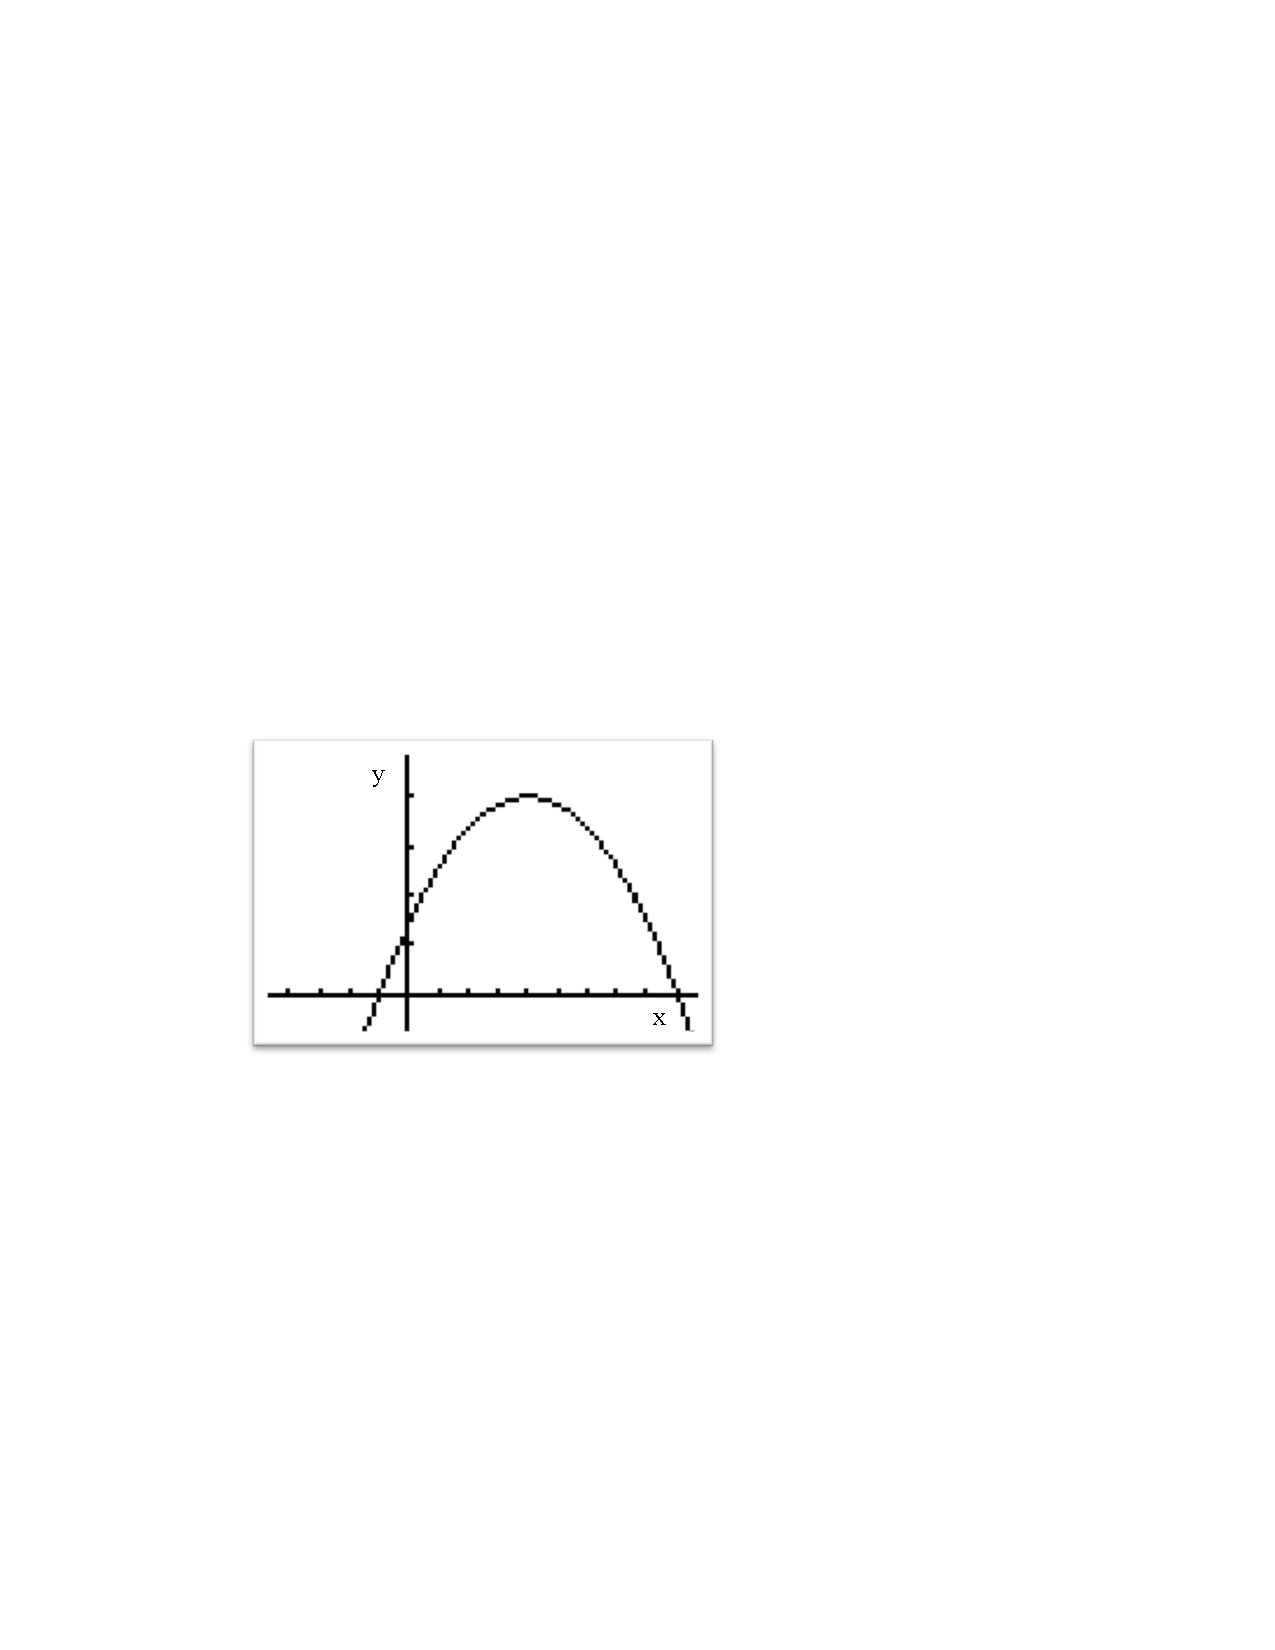
\includegraphics[scale=.4]{Figure9.png}
			\end{image}		
				\end{freeResponse}
		\item Calculate $N'(t)$.  What does $N'(t)$ represent?
			\begin{freeResponse}	
				$N'(t)=\frac{-200000(100)e^{-0.1t}}{(1+100e^{-0.1t})^2}=\frac{2000000e^{-0.1t}}{(1+100e^{-0.1t})^2}$.\\
				$N'(t)$ represents the instantaneous growth rate of the number of people getting the cold at time $t$ days.
			\end{freeResponse}

		\item Evaluate and interpret the limit $\lim_{t \to \infty} N'(t)$
			\begin{freeResponse}	
				$\lim_{t \to \infty} N'(t)=\lim_{t \to \infty}\frac{2000000e^{-0.1t}}{(1+100e^{-0.1t})^2}=\frac{2000000(0)}{(1+100(0))^2}=\frac{0}{1}=0$.\\
				There is no growth to teh cold in the long run.
			\end{freeResponse}

		\item Find the average growth rate of the number of people who have contracted the disease during the time interval $[5,6]$ (or during the fifth day after the outbreak).
			\begin{freeResponse}	
				$AVRG=\frac{N(6)-N(5)}{6-5}=N(6)-N(5)=\frac{200000}{1+100e^{-0.1(6)}}-\frac{200000}{1+100e^{-0.1(5)}} \approx 335.1$
			\end{freeResponse}

		\item Find the instantaneous growth rate of the number of people who have contracted the disease for $t=5$.
			\begin{freeResponse}	
				$N'(5)=\frac{2000000e^{-0.1(5)}}{(1+100e^{-0.1(5)})^2}$
			\end{freeResponse}

	\end{enumerate}
\end{problem}	
			
%problem5			
\begin{problem}
An oil tank is to be drained for cleaning. There are $V(t)$ gallons of oil left in the tank $t$ minutes after the draining began, where $V(t)=45(60-t)^2$.

	\begin{enumerate} 
		\item Find the average rate at which the oil drians during the first 15 minutes.
			\begin{freeResponse}
				\begin{align*}
					AR&= \frac{V(15)-V(0)}{15-0}\\
					&=\frac{45(60-15)^2-45(60-0)^2}{15-0}\\
					&=\frac{45(45)^2-45(60)^2}{15}\\
					&=\frac{45(2025-3600)}{15}\\
					&=-4725\ \text{gallons per minute}
				\end{align*}


			\end{freeResponse}
			

		\item Find the average rate at which the oil drains during the time interval $[10,15]$.
			\begin{freeResponse}
					\begin{align*}
					AR&= \frac{V(15)-V(10)}{15-10}\\
					&=\frac{45(60-15)^2-45(60-10)^2}{15-10}\\
					&=\frac{45(45)^2-45(50)^2}{5}\\
					&=\frac{45(2025-2500)}{5}\\
					&=-4275\ \text{gallons per minute}
				\end{align*}	


			\end{freeResponse}
	
		\item Find the rate at whcih the oil is flowing out of the tank 15 minutes after the draining began.
			\begin{freeResponse}
			\begin{align*}
			V'(t)&= \eval{\dd{t} 45(60-t)^2)}_{t=15}\\
			&=\eval{45 \dd{t} (60-t)^2}_{t=15}\\
			&=45\eval{\dd{t}(3600-120t+t^2)}_{t=15}\\
			&=\eval{45(-120+2t)}_{t=15}\\
			&=45(120+2(15))\\
			&=45(-120+30)\\
			&=45(-90)\\
			&=-4050\ \text{gallons per minute}
			\end{align*}
			\end{freeResponse}
		\item Find the average rate, $AR \Delta t$, at which the oil drains during the time interval:
			\begin{enumerate}
				\item $[15+ \Delta t,15],\ \text{if}\ -1< \Delta t<0$
			\begin{freeResponse}
					\begin{align*}
					AR&= \frac{V(15)-V(15+\Delta t)}{15-(15+\Delta t}\\
					&=\frac{45(60-15)^2-45(60-(15+\Delta t))^2}{-\Delta t}\\
					&=\frac{-45(45)^2+45(45-\Delta t)^2}{\Delta t}\\
					&=\frac{45(-2025+2025-90\Delta t+(\Delta t)^2)}{\Delta t}\\
					&=\frac{45(-90\Delta t+(\Delta t)^2)}{\Delta t}\\
					&=45(-90+\Delta t)\\
					&=(-4050+45\Delta t)\ \text{gallons per minute}			
					\end{align*}
			\end{freeResponse}			

				\item $[15,15+ \Delta t],\ \text{if}\ 0< \Delta t<1$
			\begin{freeResponse}
					\begin{align*}
					AR&= \frac{V(15+\Delta t)-V(15)}{15+\Delta t-15}\\
					&=\frac{45(60-(15+\Delta t))^2-45(60-15)^2}{\Delta t}\\
					&=\frac{45(45-\Delta t)^2-45(45)^2}{\Delta t}\\
					&=\frac{45(2025-90\Delta t+(\Delta t)^2)-2025}{\Delta t}\\
					&=\frac{45(-90\Delta t+(\Delta t)^2)}{\Delta t}\\
					&=45(-90+\Delta t)\\
					&=(-4050+45\Delta t)\ \text{gallons per minute}			
					\end{align*}
			\end{freeResponse}
			\end{enumerate}

		\item Use the result in part (d) to find the limit $\lim_{\Delta t \to 0} AR(\Delta t)$.  What does this limit represent?
			\begin{freeResponse}
			$\lim_{\Delta t \to 0} AR(\Delta t)=\lim_{\Delta t \to 0} (-4050+45\Delta t) =-4050$ gallons per minute.  This is the instantaneous rate at which the oil is flowing out of the tank 15 minutes after the draining began.
			\end{freeResponse}
	\end{enumerate}
	


\end{problem}


%problem6
\begin{problem}
The graph of $h(t)$ represents the height in feet of water in a pool at time $t$ minutes.
			\begin{image}
			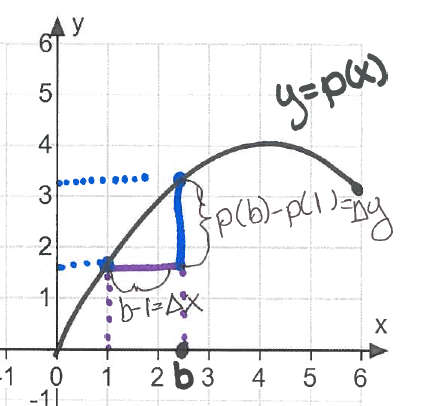
\includegraphics[scale=.5]{Figure7.png}
			\end{image}
	

	\begin{enumerate}
		\item During what time intervals is the heigh of water in the pool increasing? Decreasing?
			\begin{freeResponse}
			The height of the water in the pool is increasing when the function $h$ is increasing or has positive slope.  This is $(0,4),(7,10)$.  The height of the water is decreasing when the function $h$ is decreasing or has negative slope.  This is $(3,7),(7,12)$.
			\end{freeResponse}
		\item  Assume the rate of change of the water in the pool is $0$ when $t=0$.  For what other values of $t$ is the rate of change of the water in the pool $0$?
			\begin{freeResponse}
			The rate of the change of water in the pool is $0$ when the slope of $h$ is zero.  This is at $t=3,7,10$.
			\end{freeResponse}
		\item If $h(t)$ represents the height of the feet in water at time $t$ minutes.  What function represents the rate of change of the height over time?
			\begin{freeResponse}
				$h'(t)$, the derivative of $h(t)$.  $h'(t)$ tells us about the slope, or rate of change, of height with respect to time.
			\end{freeResponse}
		\item Sketch a graph of the rate of change of the height over time, $h'(t)$.
			\begin{freeResponse}
			We'll learn how to sketch graphs of derivatives more precisely in 4.3 but for now we can use information about the slope to help us graph $h'(t)$.\\
			First, we'll plot the points where the slope of the graph of $h(t)$ is zero.  This is at $t=0,3,7,10$.
			\begin{image}
			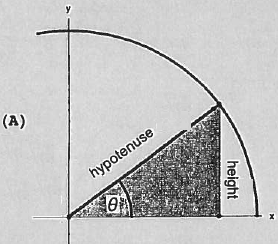
\includegraphics[scale=.4]{Figure10.png}
			\end{image}
			Next, we'll use information about whether the slope is increasing (positive) or decreasing (negative) to add tails to the zeros to indicate if the derivative should be postive or negate.  Remember, the derivative tells us about the slope. The slope of $h$ is increasing (postive) on $(0,4),(7,10)$, so $h'(t)$ is positive on $(0,4),(7,10)$.  The slope of $h$ is decreasing (negativee) on $(3,7),(7,12)$, so $h'(t)$ is negative on $(3,7),(7,12)$.
			\begin{image}
			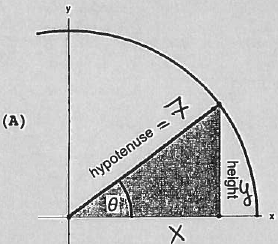
\includegraphics[scale=.4]{Figure11.png}
			\end{image}
			Finally, we'll connect our tails.  If you've already taken calculus, you may recall that we know when our derivitive $h'$ has it's highest and lowest points based on where $h$ changes concavity.  If you haven't had calculus, don't worry, we'll get there in chapter 4.  For now, just guess where you think these might be.
			\begin{image}
			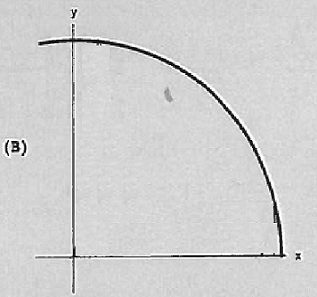
\includegraphics[scale=.4]{Figure12.png}
			\end{image}
			\end{freeResponse}
	\end{enumerate}

\end{problem}






\end{document} 


















